
   %%%%%%%%%%%%%%%%%%%%%%%
 %%%  NOAH'S SUPER COOL  %%%
%%%%      ACADEMIC       %%%%
 %%%   LATEX TEMPLATE    %%%
   %%%%%%%%%%%%%%%%%%%%%%%

\documentclass[12pt]{article}
\usepackage[letterpaper]{geometry}
\geometry{top=1in, bottom=1in, left=1in, right=1in}
\usepackage{fontspec}
\usepackage{tgtermes}
\usepackage{hanging}
\setmainfont[
 ItalicFont={texgyretermes-italic.otf},
 BoldFont={texgyretermes-bold.otf},
 ]{texgyretermes-regular.otf}
\usepackage{setspace}
\doublespacing
\usepackage{graphicx}
\graphicspath{ {./} }

\begin{document}

% Title Page
\pagenumbering{gobble} % remove page numbers
\begin{center}
\topskip0pt
\vspace*{\fill}
Friction Lab 6 \\ Noah Dinan \\ PHY 1110 - Mayer \\ \today \\
\vspace*{\fill}
\end{center}

\newpage
\pagenumbering{arabic} % resume page numbering

\setlength{\parindent}{0in}

\textbf{Results}

As the sled is dragged along the board, the ratio between the force of kinetic friction and the normal force
results in the coefficiient of kinetic friction, a number between 0 and 1.

The largest likely source of error was in the measurements for length taken with a ruler.
Another source of error was that the weights used did not weigh exactly what they were labeled.

Below is the equation to represent kinetic friction

\[ \mu_k = \frac{f_k}{N} \]

For this experiment, the coefficient of static friction is not constant because the sled accelerates as the block falls.
We measured the distance between the two photogates and found it was $ 21.6 cm $, the distance between the starting position
and the first photogate is $ 5.0 cm $.

We measured the weight of the sled to be $ 433.1 $ grams using a digital scale. Using this mass we calculated the normal force.

\[ F_N = mg = 0.433 * 9.81 = 4.25N \]

\newpage

We used the value of the normal force to graph $\mu_k$ against $\overline{v}$ shown below.

\vspace{0.5cm}

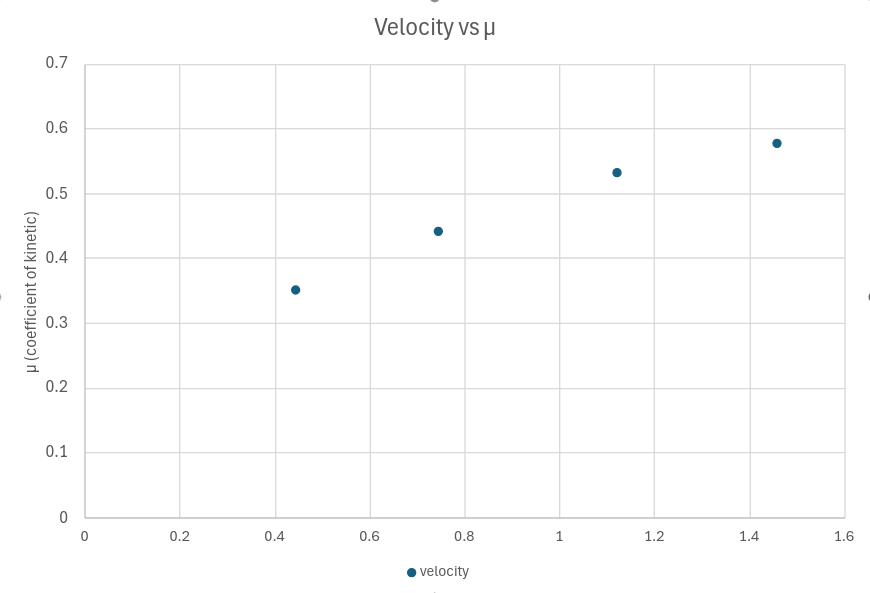
\includegraphics[scale=0.53]{graph.png}

\textbf{Conclusions}

The coefficient of friction is not independent of the speed of the sled, based on the graph above,
as speed increases, $\mu_k$ increases also.
The coefficient of friction likely depends on speed because as an object is moving quicker and quicker
friction is less impactful. The value of the coefficient of friction is dependent on the velocity of the object.

\end{document}
